%%%%%%%%%%%%%%%%%%%%%%%%%%%%%%%%%%%%%%%%%%%
%%%%%%%%%%%%%%%%%%%%%%%%%%%%%%%%%%%%%%%%%%%
%%%%%%%%%%%%%%% CHAPTER 08 %%%%%%%%%%%%%%%%


\section{Função de transferência}

\frame{
\frametitle{Introdução}
\begin{block}{Contextualização}
Na teoria de controle, as \textbf{funções de transferência} são comumente utilizadas para caracterizar as \textbf{relações de entrada e de saída} de componentes ou de sistemas que podem ser descritos por equações diferenciais lineares invariantes no tempo.
\end{block}
}

\frame{
\frametitle{Introdução}
\begin{block}{Contextualização}
Essa função permitirá a separação da entrada, do sistema e da saída em três partes separadas e distintas, diferentemente do que ocorre com a equação diferencial.
\begin{itemize}
    \item A função também permitirá combinar algebricamente representações matemáticas de \textbf{subsistemas} para produzir uma representação do sistema como um todo.
\end{itemize}
\end{block}
\vspace{0.2cm}
\centerline{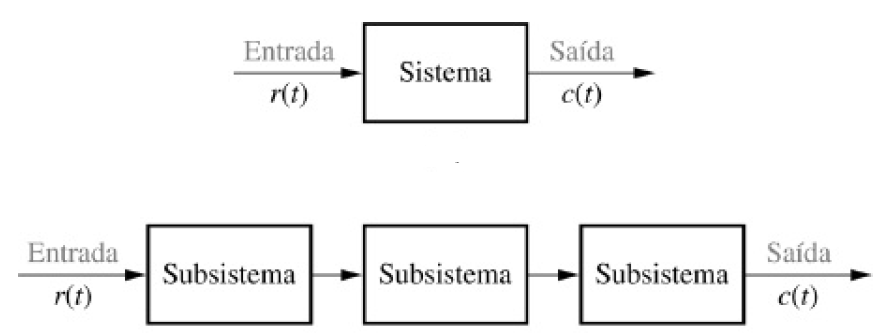
\includegraphics[width=0.8\linewidth]{Figuras/Ch08/fig1.PNG}}
}

\frame{
\frametitle{Introdução}
\begin{block}{Definição}
Seja uma equação diferencial geral de ordem $n$, linear e invariante no tempo,
\begin{equation*}
\begin{split}
a_n \dfrac{d^n c(t)}{dt^n} + a_{n-1} \dfrac{d^{n-1} c(t)}{dt^{n-1}} + \cdots + a_0 c(t) = \\
= b_m \dfrac{d^m r(t)}{dt^m} + b_{m-1} \dfrac{d^{m-1} r(t)}{dt^{m-1}} + \cdots + b_0 r(t)
\end{split}
\end{equation*}
em que $c(t)$ é a \textbf{saída}, $r(t)$ é a \textbf{entrada} e os coeficientes $a_i$ e $b_i$ e a forma da ED representam o \textbf{sistema}. Aplicando a T.L., temos:
\begin{equation*}
\begin{split}
a_n s^n C(s) + a_{n-1} s^{n-1} C(s) + \cdots + a_0 C(s) + \text{CI} = \\
= b_m s^m R(s) + b_{m-1} s^{m-1} R(s) + \cdots + b_0 R(s) + \text{CI}
\end{split}
\end{equation*}
Perceba que a equação acima é \textbf{puramente algébrica}. Se admitirmos que \textbf{todas as condições inicias são nulas}, temos:
$$(a_n s^n + a_{n-1} s^{n-1} + \cdots + a_0)C(s) = ( b_m s^m + b_{m-1} s^{m-1} + \cdots + b_0)R(s)$$
\end{block}
}

\frame{
\frametitle{Introdução}
\begin{block}{Definição}
Agora formando a \textbf{razão} da transformada da saída, $C(s)$, divida pela transformada da entrada, $R(s)$, obtemos:
$$\dfrac{C(s)}{R(s)} = G(s) = \dfrac{b_m s^m + b_{m-1} s^{m-1} + \cdots + b_0}{a_n s^n + a_{n-1} s^{n-1} + \cdots + a_0}$$
Observe que esta equação separa a \textbf{saída}, $C(s)$, a \textbf{entrada}, $R(s)$, e o sistema, que é a razão entre polinômios em $s$ do lado direito da igualdade.
\end{block}
\centerline{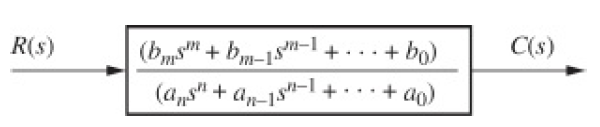
\includegraphics[width=0.6\linewidth]{Figuras/Ch08/fig2.PNG}}
}

\frame{
\frametitle{Introdução}
\begin{block}{Definição formal}
A \textbf{função de transferência} de um sistema representado por uma equação diferencial linear invariante no tempo é definida como a \textbf{relação} entre a transformada de Laplace da \textbf{saída} (função de resposta - \textit{response function}) e a transformada de Laplace da \textbf{entrada} (função de excitação - \textit{driving function}), admitindo-se todas as \textbf{condições inicias nulas}.
\begin{itemize}
    \item Se a maior potência de $s$ no denominador da função de transferência for igual a $n$, o sistema será denominado sistema de ordem $n$.
    \item Observe que o denominador da função de transferência é idêntico ao \textbf{polinômio característico} da equação diferencial.
\end{itemize}
\end{block}
}

\frame{
\frametitle{Comentários}
\begin{block}{Comentários sobre a função de transferência}
\begin{enumerate}
    \item A função de transferência de um sistema é um \textbf{modelo matemático} que constitui um método operacional para expressar a equação diferencial que \textbf{relaciona} a variável de saída à variável de entrada.
    \item A função de transferência é uma \textbf{propriedade inerente do sistema}, independentemente da magnitude e da natureza da função de entrada ou de excitação.
    \item A função de transferência inclui as unidades necessárias para relacionar a entrada à saída; entretanto, \textbf{não} fornece nenhuma informação relativa à \textbf{estrutura física do sistema}.
    \item Se a função de transferência de um sistema for conhecida, \textbf{a saída ou a resposta poderá ser estudada} para várias maneiras de entrada, visando ao entendimento da natureza do sistema.
    \item Se a função de transferência de um sistema não for conhecida, ela pode ser determinada \textbf{experimentalmente} com o auxílio de entradas conhecidas e do estudo das respectivas respostas do sistema.
\end{enumerate}
\end{block}
}

\cprotect\frame{
\frametitle{\MATLAB}
\begin{block}{}
\begin{verbatim}
>>tf(num,den)
\end{verbatim}
retorna a função de transferência expressa como um polinômio do numerador $\bm{num}$ dividido por um polinômio do denominador $\bm{den}$.\\
\end{block}
\centerline{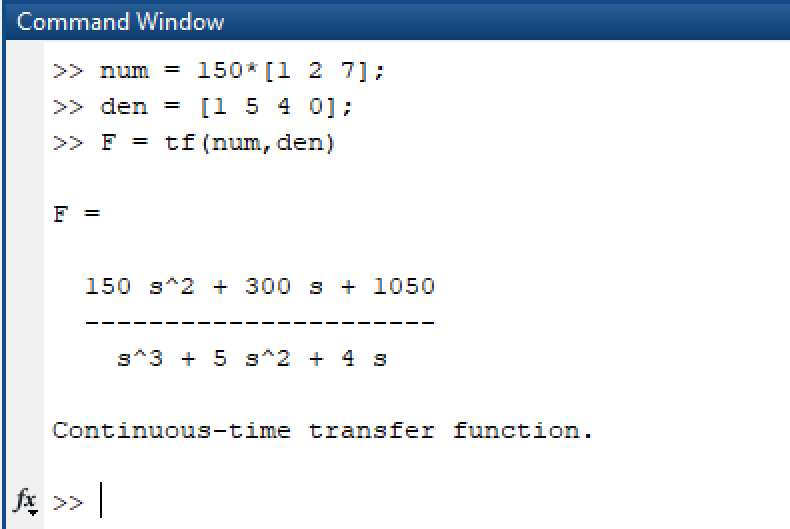
\includegraphics[width=0.7\linewidth]{Figuras/Ch08/fig3.PNG}}
}

\frame{
\frametitle{Exemplo $\#01$ - função de transferência de uma equação diferencial}
\begin{block}{}
Obtenha a função de transferência representada por
$$\dfrac{dc(t)}{dt} + 2c(t) = r(t)$$

\vspace{0.2cm}

\textbf{Solução}: Aplicando a T.L. a ambos os lados da equação, admitindo condições inicias nulas, temos
$$sC(s) + 2C(s) = R(s)$$
$$G(s) = \dfrac{C(s)}{R(s)} = \dfrac{1}{s+2}$$
\end{block}
}

\frame{
\frametitle{Exemplo $\#02$ - resposta do sistema a partir da F.T.}
\begin{block}{}
Usando o resultado do exemplo $\#01$, obtenha a resposta $c(t)$ para uma resposta $r(t) = u(t)$ (degrau unitário).

\vspace{0.2cm}

\textbf{Solução}: 
$$C(s) = R(s)G(s) = \dfrac{1}{s(s+2)}$$
Expandindo em frações parciais, obtemos:
$$C(s) = \dfrac{0,5}{s} - \dfrac{0,5}{s+2}$$
Utilizando a T.I.L., temos:
$$c(t) = 0,5(1 - e^{-2t})$$
\end{block}
}

\cprotect\frame{
\frametitle{\MATLAB}
\begin{block}{}
\begin{verbatim}
>>plot(t,f,s)
\end{verbatim}
representa graficamente a função do tempo onde $\bm{t}$ é a variável independente, $\bm{f}$ é a variável dependente e $\bm{s}$ é uma cadeia de caracteres opcionais (cor, marcador, etc). \\
\vspace{0.2cm}
\textbf{Exemplo}: represente graficamente o resultado do exemplo $\#02$ para $t$ variando de 0 a 1 em intervalos de 0,01 s. Utilize $\bm{s}$ como $\bm{'r'}$ para que o gráfico seja exibido em vermelho.
\end{block}
\centerline{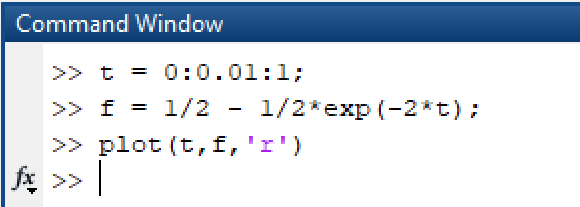
\includegraphics[width=0.6\linewidth]{Figuras/Ch08/fig4.PNG}}
}

\frame{
\frametitle{\MATLAB}
\centerline{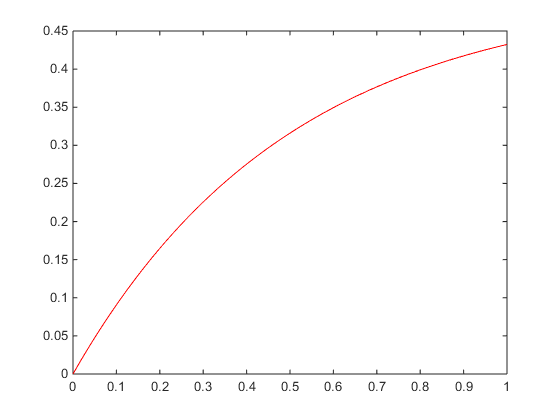
\includegraphics[width=0.9\linewidth]{Figuras/Ch08/fig5.png}}
}

\frame{
\frametitle{Exemplo $\#03$ - sistema massa-mola-amortecedor}
\centerline{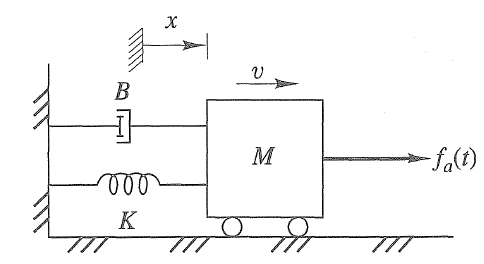
\includegraphics[width=0.5\linewidth]{Figuras/Ch05/fig8.PNG}}
\begin{block}{Revisitando o problema...}
$$M\ddot{x} + B\dot{x} + Kx = f_a(t)$$
\end{block}
}

\frame{
\frametitle{Exemplo $\#03$ - sistema massa-mola-amortecedor}
\begin{block}{Função de transferência}
Aplicando a T.L., admitindo condições iniciais nulas,
$$Ms^2 X(s) + Bs X(s) + K X(s) = F_a(s)$$
Rearranjando os termos, temos:
$$(Ms^2 + Bs + K)X(s) = F_a(s)$$
Resolvendo para a função de transferência, resulta
$$G(s) = \dfrac{X(s)}{F_a(s)} = \dfrac{1}{Ms^2 + Bs + K}$$
\end{block}
}

\frame{
\frametitle{Exemplo $\#04$ - sistema com duas massas interconectadas}
\centerline{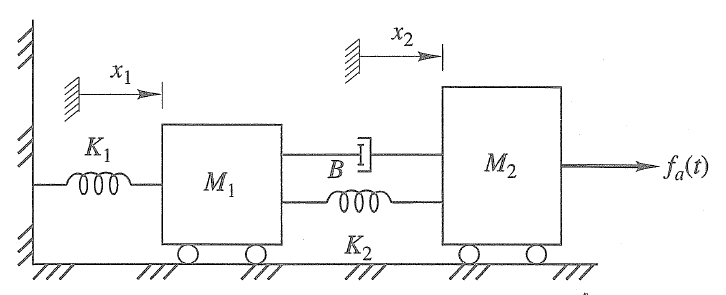
\includegraphics[width=0.6\linewidth]{Figuras/Ch05/fig10.PNG}}
\begin{block}{Revisitando o problema...}
\begin{equation*}
\begin{cases}
M_1\ddot{x}_1 + B\dot{x}_1 + (K_1 + K_2)x_1 - B\dot{x}_2 - K_2x_2= 0 \\
-B\dot{x}_1 - K_2x_1 + M_2\ddot{x}_2 + B\dot{x}_2 + K_2x_2 = f_a(t)
\end{cases}
\end{equation*}
\end{block}
}

\frame{
\frametitle{Exemplo $\#04$ - sistema com duas massas interconectadas}
\begin{block}{Função de transferência}
Aplicando a T.L., admitindo condições iniciais nulas,
\begin{equation*}
\begin{cases}
M_1s^2 X_1(s) + Bs X_1(s) + (K_1 + K_2) X_1(s) - Bs X_2(s) - K_2 X_2(s) = 0 \\
-Bs X_1(s) - K_2 X_1(s) + M_2s^2 X_2(s) + Bs X_2(s) + K_2 X_2(s) = F_a(s)
\end{cases}
\end{equation*}
Rearranjando os termos, temos:
\begin{equation*}
\begin{cases}
[M_1s^2 + Bs + (K_1 + K_2)] X_1(s) - [Bs + K_2] X_2(s) = 0 \\
-[Bs + K_2] X_1(s) + [M_2s^2 + Bs + K_2] X_2(s) = F_a(s)
\end{cases}
\end{equation*}
\end{block}
}

\frame{
\frametitle{Exemplo $\#04$ - sistema com duas massas interconectadas}
\begin{block}{Função de transferência}
Isolando $X_1(s)$ da primeira equação anterior, temos
$$X_1(s) = \dfrac{[Bs + K_2] X_2(s)}{M_1s^2 + Bs + (K_1 + K_2)}$$
Substituindo esta nova equação na segunda equação anterior, e resolvendo para $X_2(s)$, obtemos:
$$-[Bs + K_2] \dfrac{[Bs + K_2] X_2(s)}{M_1s^2 + Bs + (K_1 + K_2)} + [M_2s^2 + Bs + K_2] X_2(s) = F_a(s)$$
\begin{equation*}
\begin{split}
[M_2s^2 + Bs + K_2][M_1s^2 + Bs + (K_1 + K_2)]X_2(s) -[Bs + K_2]^2 X_2(s) \\
= [M_1s^2 + Bs + (K_1 + K_2)] F_a(s)
\end{split}
\end{equation*}
Deste modo,
$$\dfrac{X_2(s)}{F_a(s)} = \dfrac{M_1s^2 + Bs + (K_1 + K_2)}{[M_2s^2 + Bs + K_2][M_1s^2 + Bs + (K_1 + K_2)] -[Bs + K_2]^2}$$
\end{block}
}

\frame{
\frametitle{Exemplo $\#04$ - sistema com duas massas interconectadas}
\begin{block}{Função de transferência}
Isolando $X_2(s)$ da função de transferência anterior, obtemos
$$X_2(s) = F_a(s) \cdot \dfrac{M_1s^2 + Bs + (K_1 + K_2)}{[M_2s^2 + Bs + K_2][M_1s^2 + Bs + (K_1 + K_2)] -[Bs + K_2]^2}$$
Substituindo em
$$X_1(s) = \dfrac{[Bs + K_2] X_2(s)}{M_1s^2 + Bs + (K_1 + K_2)}$$
temos
$$X_1(s) = \dfrac{[Bs + K_2] \cdot F_a(s)}{[M_2s^2 + Bs + K_2][M_1s^2 + Bs + (K_1 + K_2)] -[Bs + K_2]^2}$$
Deste modo,
$$\dfrac{X_1(s)}{F_a(s)} = \dfrac{Bs + K_2}{[M_2s^2 + Bs + K_2][M_1s^2 + Bs + (K_1 + K_2)] -[Bs + K_2]^2}$$
\end{block}
}

\frame{
\frametitle{Exemplo $\#05$ - sistema rotacional simples}
\centerline{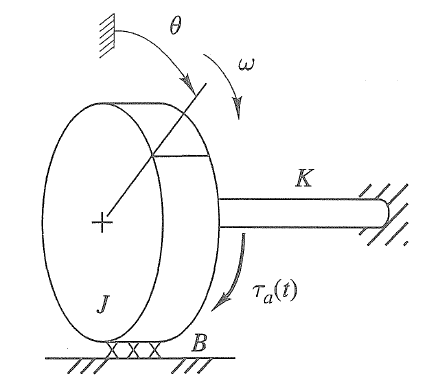
\includegraphics[width=0.4\linewidth]{Figuras/Ch06/fig8.PNG}}
\begin{block}{Revisitando o problema...}
$$J\ddot{\theta} + B\dot{\theta} + K\theta = \tau_a(t)$$
\end{block}
}

\frame{
\frametitle{Exemplo $\#05$ - sistema rotacional simples}
\begin{block}{Função de transferência}
Aplicando a T.L., admitindo condições iniciais nulas,
$$Js^2 \Theta(s) + Bs \Theta(s) + K \Theta(s) = \tau_a(s)$$
Rearranjando os termos, temos:
$$(Js^2 + Bs + K)\Theta(s) = \tau_a(s)$$
Resolvendo para a função de transferência, resulta
$$G(s) = \dfrac{\Theta(s)}{\tau_a(s)} = \dfrac{1}{Js^2 + Bs + K}$$
\end{block}
}

\frame{
\frametitle{Exemplo $\#06$ - sistema rotacional com dois discos interconectados}
\centerline{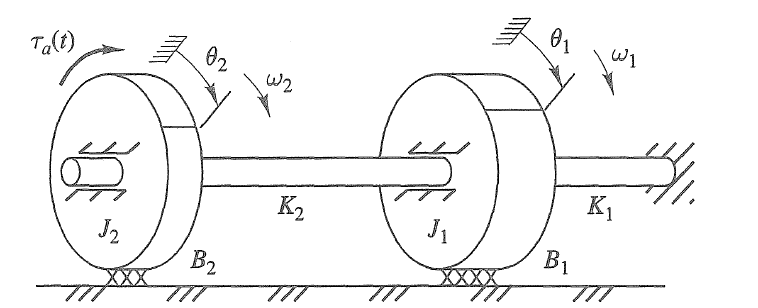
\includegraphics[width=0.7\linewidth]{Figuras/Ch06/fig10.PNG}}
\begin{block}{Revisitando o problema...}
\begin{equation*}
\begin{cases}
J_1\ddot{\theta}_1 + B_1\dot{\theta}_1 + (K_1 + K_2)\theta_1 - K_2\theta_2 = 0 \\
-K_2\theta_1 + J_2\ddot{\theta}_2 + B_2\dot{\theta}_2 + K_2\theta_2= \tau_a(t)
\end{cases}
\end{equation*}
\end{block}
}

\frame{
\frametitle{Exemplo $\#06$ - sistema rotacional com dois discos interconectados}
\begin{block}{Função de transferência}
Aplicando a T.L., admitindo condições iniciais nulas,
\begin{equation*}
\begin{cases}
J_1s^2 \Theta_1(s) + B_1s \Theta_1(s) + (K_1 + K_2) \Theta_1(s) - K_2 \Theta_2(s) = 0 \\
- K_2 \Theta_1(s) + J_2s^2 \Theta_2(s) + B_2s \Theta_2(s) + K_2 \Theta_2(s) = \tau_a(s)
\end{cases}
\end{equation*}
Rearranjando os termos, temos:
\begin{equation*}
\begin{cases}
[J_1s^2 + B_1s + (K_1 + K_2)] \Theta_1(s) - K_2 \Theta_2(s) = 0 \\
- K_2 \Theta_1(s) + [J_2s^2 + B_2s + K_2] \Theta_2(s) = \tau_a(s)
\end{cases}
\end{equation*}
\end{block}
}

\frame{
\frametitle{Exemplo $\#06$ - sistema rotacional com dois discos interconectados}
\begin{block}{Função de transferência}
Isolando $\Theta_1(s)$ da primeira equação anterior, temos
$$\Theta_1(s) = \dfrac{K_2 \Theta_2(s)}{J_1s^2 + B_1s + (K_1 + K_2)}$$
Substituindo esta nova equação na segunda equação anterior, e resolvendo para $\Theta_2(s)$, obtemos:
$$-K_2 \dfrac{K_2 \Theta_2(s)}{J_1s^2 + B_1s + (K_1 + K_2)} + [J_2s^2 + B_2s + K_2] \Theta_2(s) = \tau_a(s)$$
\begin{equation*}
\begin{split}
[J_2s^2 + B_2s + K_2][J_1s^2 + B_1s + (K_1 + K_2)]\Theta_2(s) -K_2^2 \Theta_2(s) \\
= [J_1s^2 + B_1s + (K_1 + K_2)] \tau_a(s)
\end{split}
\end{equation*}
Deste modo,
$$\dfrac{\Theta_2(s)}{\tau_a(s)} = \dfrac{J_1s^2 + B_1s + (K_1 + K_2)}{[J_2s^2 + B_2s + K_2][J_1s^2 + B_1s + (K_1 + K_2)] - K_2^2}$$
\end{block}
}

\frame{
\frametitle{Exemplo $\#06$ - sistema rotacional com dois discos interconectados}
\begin{block}{Função de transferência}
Isolando $\Theta_2(s)$ da função de transferência anterior, obtemos
$$\Theta_2(s) = \tau_a(s) \cdot \dfrac{J_1s^2 + B_1s + (K_1 + K_2)}{[J_2s^2 + B_2s + K_2][J_1s^2 + B_1s + (K_1 + K_2)] - K_2^2}$$
Substituindo em
$$\Theta_1(s) = \dfrac{K_2 \Theta_2(s)}{J_1s^2 + B_1s + (K_1 + K_2)}$$
temos
$$\Theta_1(s) = \dfrac{K_2 \cdot \tau_a(s)}{[J_2s^2 + B_2s + K_2][J_1s^2 + B_1s + (K_1 + K_2)] -K_2^2}$$
Deste modo,
$$\dfrac{\Theta_1(s)}{\tau_a(s)} = \dfrac{K_2}{[J_2s^2 + B_2s + K_2][J_1s^2 + B_1s + (K_1 + K_2)] - K_2^2}$$
\end{block}
}

\frame{
\frametitle{Exemplo $\#07$ - circuito RLC série}
\centerline{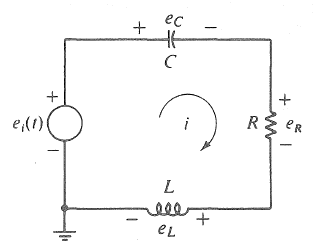
\includegraphics[width=0.5\linewidth]{Figuras/Ch07/fig5.PNG}}
\begin{block}{Revisitando o problema...}
$$L\dfrac{d^2i}{dt^2} + R\dfrac{di}{dt} + \dfrac{1}{C}i = \dot{e}_i$$
\end{block}
}

\frame{
\frametitle{Exemplo $\#07$ - circuito RLC série}
\begin{block}{Função de transferência}
Aplicando a T.L., admitindo condições iniciais nulas,
$$Ls^2 I(s) + Rs I(s) + \dfrac{1}{C} I(s) = sE_i(s)$$
Rearranjando os termos, temos:
$$\Big(Ls^2 + Rs + \dfrac{1}{C}\Big)I(s) = sE_i(s)$$
Resolvendo para a função de transferência, resulta
$$G(s) = \dfrac{I(s)}{E_i(s)} = \dfrac{s}{Ls^2 + Rs + \dfrac{1}{C}}$$
\end{block}
}

\frame{
\frametitle{Exemplo $\#08$ - circuito RLC série (outra variável de saída)}
\centerline{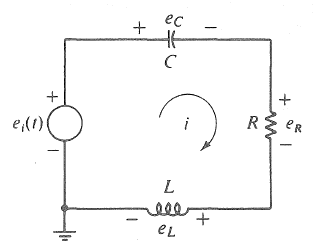
\includegraphics[width=0.5\linewidth]{Figuras/Ch07/fig5.PNG}}
\begin{block}{Revisitando o problema...}
$$G(s) = \dfrac{I(s)}{E_i(s)} = \dfrac{s}{Ls^2 + Rs + \dfrac{1}{C}}$$
\end{block}
}

\frame{
\frametitle{Exemplo $\#08$ - circuito RLC série (outra variável de saída)}
\begin{block}{Função de transferência}
Suponha que agora queiramos saber a função de transferência que relaciona a tensão no capacitor ($e_C$) com a tensão de entrada. Sabemos que,
$$e_c(t) = e(t_0) + \dfrac{1}{C}\int_{t_0}^{t} i(\lambda) d\lambda$$
Deste modo,
$$E_C(s) = \dfrac{1}{Cs}I(s)$$
Portanto,
$$G'(s) = \dfrac{E_C(s)}{I(s)} = \dfrac{1}{Cs}$$
Resolvendo para a função de transferência, resulta
$$H(s) = G(s) \cdot G'(s) = \dfrac{I(s)}{E_i(s)} \cdot \dfrac{E_C(s)}{I(s)} = \dfrac{E_C(s)}{E_i(s)} = \dfrac{1}{LCs^2 + RCs + 1}$$
\end{block}
}

\frame{
\frametitle{Exercícios}
\begin{block}{}
01. Revisite todos os exercícios propostos (final de capítulo) de modelagem de sistemas mecânicos de translação, sistemas mecânicos de rotação e sistemas elétricos; e determine todas as possíveis funções de transferência. 
\end{block}
}

\frame{
\frametitle{Referências e exercícios complementares}
\begin{itemize}
\item  NISE, Norman S. Engenharia de Sistemas de Controle, 7 ed. LTC, 2017.
\end{itemize}
\centering{\alert{Página 77 - \textbf{Capítulo 2}}} \\
}